\documentclass{article}
\usepackage{caption}
\usepackage{titlesec}

% \usepackage{listings}

\titleformat{\subsection}
  {\normalfont\large\bfseries}{\alph{subsection})}{1em}{}

% Language setting
% Replace `english' with e.g. `spanish' to change the document language
\usepackage[english]{babel}

% Set page size and margins
% Replace `letterpaper' with `a4paper' for UK/EU standard size
\usepackage[letterpaper,top=2cm,bottom=2cm,left=3cm,right=3cm,marginparwidth=1.75cm]{geometry}


% Useful packages
\usepackage{amsmath}
\usepackage{graphicx}
\usepackage[colorlinks=true, allcolors=blue]{hyperref}

\title{Assignment 1}
\author{Kappala Hemanth Krishna, 2021CS10102 \\ Koduru Suchith, 2021CS10572}


\date{August, 13th 2023}

\begin{document}
\maketitle

\section{Network Analysis}

\begin{itemize}
\item I ran traceroute with wifi network and 4G network. 



\begin{center}
\centering
    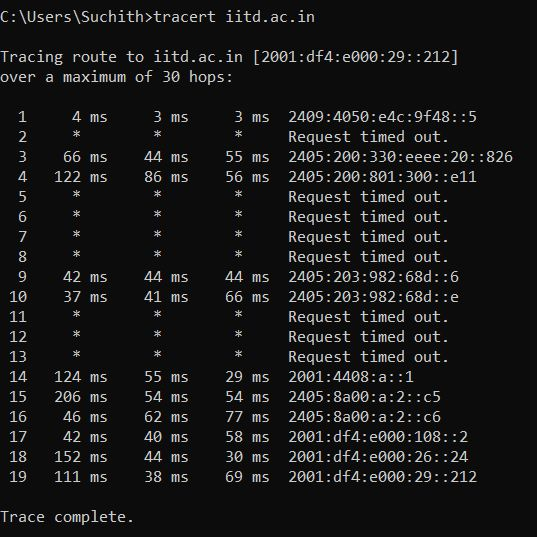
\includegraphics[width=0.90\textwidth]{4G_ip6.jpg}
    \captionof{figure}{Results for the \texttt{tracert iitd.ac.in} command via 4G network.}
\end{center}

\begin{center}
\centering
    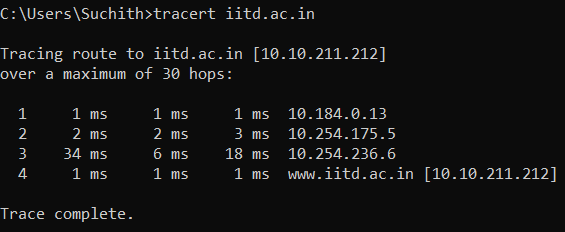
\includegraphics[width=0.90\textwidth]{wifi_ip4.png}
    \captionof{figure}{Results for the \texttt{tracert iitd.ac.in} command via IITD wifi.}
\end{center}
\end{itemize}


\begin{itemize}
\item When I run traceroute command via 4G network, I got path that is default to IPv6. We can force traceroute to use IPv4 by adding -4 option in the command, then the command will be "tracert -4 iitd.ac.in".
\begin{center}
\centering
    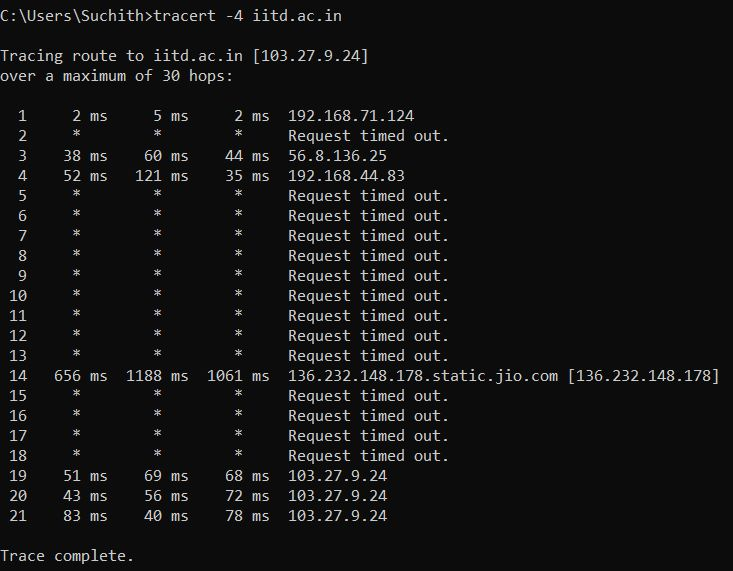
\includegraphics[width=0.90\textwidth]{4G_ip4.jpg}
    \captionof{figure}{Results for the \texttt{tracert -4 iitd.ac.in} command via 4G network.}
\end{center}
\item In the path via IITD wifi, all the ip's in the path are private IP address, since I ran the command by using wifi so the tracert took the nearest routers in the campus which are private ip's of IIT Delhi campus.
\item In the path via 4G network, only 1st and 3rd ip's in the path are private ip's, they are probably private ip's of jio network which are near to the campus.
\item Maximum size of ping packets that I am able to send via 4G network connection is "1452". It was varying when I tried in different times, I also got it as "1472" otherday.
\end{itemize}



\section{Replicating traceroute with ping}
\begin{itemize} 

\item We can replicate traceroute functionality using some option of the ping and loop.
\item First I used ping command directly to the destination to get ip address of the destination.
\item Then I initialized a ttl value with 1, empty list 'ans' and a boolean value "reached" and used it to loop through while loop, and change boolean value of "reached" to True, then the loop will stop.
\item In the every iteration of while loop, I ran the ping command with options '-n' which specifies no of packets, '-i' which specifies ttl value to get the ip address which it reached in the middle of path with that ttl value. 
\item If the packets are blocked by ISP and I didn't get intermediate ip address I stored 'Request timed out' for that ttl, and stored the ip address for remaining.
\item After getting intermediate ip addresses, I sent 3 packets using ping command and noted the RTT values for those. If the ip address matched with the destination ip address I changed the boolean value of 'reached' to True.
\item Finally in every iteration I stored the ip address and 3 RTT's in the 'ans' list and incremented the ttl value by 1.


% \begin{lstlisting}[language=Python, caption=My Python Script]
% # Your Python code here
% def hello_world():
%     print("Hello, world!")
% \end{lstlisting}

\end{itemize}

\section{Internet architecture}


\subsection{}
\begin{itemize}
    \item \textbf{Table 1: No of Hops}
\end{itemize}


    \begin{tabular}{|c|c|c|c|}
  \hline
  \textbf{Server Name} & \textbf{Localhost} & \textbf{Germany} & \textbf{US(NYC)}\\
  \hline
  iitd.ac.in & 14hops & 18hops & 15hops \\
  \hline
   www.utah.edu & NA  & NA& 20hops (Ipv4)     \\
  \hline
   www.uct.ac.za & NA & NA & NA\\
  \hline
  www.google.com & 13hops & 11hops & 24hops \\
  \hline
  www.facebook.com & 10hops & 11hops & 8hops \\
  \hline
\end{tabular}
\begin{itemize}
    \item NA means \textbf{not reached} (more than 30 hops)
    \item Geographical proximity can indeed result in fewer hops between traceroute sources and destinations. If two points are geographically close, there might be a more direct network path between them, potentially reducing the number of intermediate routers and hops.
    \item In the above table we can see that US(NYT)-IITD took less hops(15hops) compared to Germany-IITD even though Germany is geographically nearer than US(NYC).
    \item Yes,Google and Facebook, being two of the largest and most well-connected internet entities, often have robust network infrastructures and distributed data centers. This can lead to optimized routing and potentially fewer hops required to reach their servers. Additionally, they might have peering agreements with major ISPs, allowing for more direct paths.


\end{itemize}

\subsection{}



\begin{itemize}
   \item \textbf{Table 2 : Latency}

\begin{tabular}{|c|c|c|c|}
  \hline
  \textbf{Server Name} & \textbf{Localhost} & \textbf{Germany} & \textbf{US}\\
  \hline
  iitd.ac.in & 46ms & 161.279ms & 275.897ms \\
  \hline
   www.utah.edu & NA  & NA & 55.530ms (Ipv4)     \\
  \hline
   www.uct.ac.za & NA & NA & NA\\
  \hline
  www.google.com & 72.845ms & 3.116ms & 6.795ms \\
  \hline
  www.facebook.com & 90.943 &9.386 & 0.623ms \\
  \hline
\end{tabular}
\item \textbf{Latency and Hop Count:}In general, as the number of hops increases, the latency tends to increase as well. This is because each router along the path introduces processing time and potential transmission delays.Each router processes the packet, makes a forwarding decision, and introduces a certain amount of delay before passing it to the next hop. This cumulative processing time contributes to overall latency.
\item\textbf{Routing Efficiency :}The routing decisions made by routers can influence the overall latency. Inefficient routing can lead to longer paths and higher latency.Sometimes, network congestion or suboptimal routing decisions can lead to higher latencies even with a smaller number of hops.


\end{itemize}
\subsection{}
\begin{itemize}
    \item iitd.ac.in, www.utah.edu,www.uct.ac.za are resloved to the same IP address irrespective of the traceroute source and www.google.com and facebook.com resolved to different IP addresses. Although the servers of educational institutions are giving the same IP address, if we run traceroute command from IITD via Institute wifi, we get another IP address which is private since the network is also private.
    \item For the webservers of large content providers, there are multiple servers present across the globe. So we are getting different IP addresses for them when we run traceroute command from different source.


\end{itemize}
\subsection{}
\begin{itemize}
    \item \textbf{Geographical Diversity:} Some paths might take more direct routes based on geographical proximity, while others might route through different locations due to network peering agreements.Here due to geographical proximity the paths are longer. Longer paths have higher hops.
    \item\textbf{Example:} NYC to faceboook(US) is 8 hops and NYC to facebook(India) is 18hops. geogrpahically facebook (India) is farther from facebook(US) which results in more hops than facebook(US).
\end{itemize}
\subsection{}
\begin{itemize}
    \item Buenos Aires, AR for this country traceroute didn't reach destination for google and facebook.
    \item For other countries servers, traceroute path is complete mostly for google and facebook. So I didn't find any other country whose ISP is not directly peered with google and facebook.
\end{itemize}

\section{Packet Analysis}
\subsection{DNS filter}
\paragraph{} we did packet trace for www.iitd.ac.in and applied dns filter.THe request-response time for A record(which resolves IP address)is 3.312ms and for https is 2.064ms.
\subsection{HTTP filter}
\paragraph{} observations on apllying http filter to the act4d.iitd.ac.in
\begin{itemize}
    \item number of http requests tha genereted are 12.
    \item \textbf{Multiple Requests :} It has generated multiple http requests to fetch all the js,css,html files.
    \item\textbf{Rendering Process :} Browser has started rendering the page as soon as it recieved the html file, they will pause rendering if they encounter external resources(images,stylesheets,scripts)referenced in HTML until those are fetched and loaded.
    \item\textbf{Paraller Fetching :} Browsers can fetch resources in parallel to improve page loading speed. This allows browser to efficiently retrieve multiple resources simultaneously,making use of available network bandwith
    \item\textbf{asynchronous Loding :}To optimize performance, web developers often use techniques like asynchronous loading of scripts and lazy loading of images. This means some resources might be fetched after the main page is displayed, further improving perceived page load times.
    
\end{itemize}
\subsection{TCP connection}
\begin{itemize}
    \item \textbf{No of TCP connections :} 6
    \item \textbf{Number of TCP Connections vs. Number of HTTP Requests:}No of TCP connections and HTTP requests we got in the previous part are not same. Because here a single TCP connection can serve multiple HTTP requests using techniwues like HTTP/1.1 pipeling.
    \item \textbf{Content Objects Over the Same TCP Connection:}Yes, content objects can be fetched over the same TCP connection. Modern browsers and web servers often use techniques to optimize performance, such as keeping connections open and reusing them for fetching multiple resources. This reduces the overhead of establishing new TCP connections for each resource.
\end{itemize}
\subsection{Indian Express}
\begin{itemize}
    \item \textbf{HTTP Traffic:} There is HTTP traffic. which sent a request to http:/indianexpress.com/
    \item\textbf{Content:}there is only one html file.
    \item\textbf{Analysis:}What happende is browser is making HTTP requests to the websites server for various resiources,including HTML files(whihc define the structres of the web page). These resources are fetched using HTTP GET requests. Browser then processses this content to render the webpage correctly.
\end{itemize}


\end{document}